%-----------------------------------------------------------------------------%
\chapter{HASIL PENELITIAN DAN PEMBAHASAN}
%-----------------------------------------------------------------------------%

%
\vspace{4.5pt}
\begin{flushleft}
    \section{Hasil Penelitian}
    \subsection{Data Hasil Observasi}
\vspace{5cm}
\begin{figure}[ht]
	\centering
	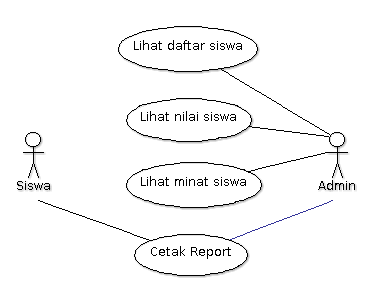
\includegraphics[width=10cm]{images/UseCaseDiagramSistemSaatIni}
	\caption{Gambar Observasi}
\end{figure}
Peneliti mengamati kebutuhan sensor dan kontrol yang diperlukan petani untuk diaplikasikan pada lahannya. 
% \caption{Gambar Observasi}
    \section{Analisis Hasil Penelitian}

\end{flushleft}

\vspace{5cm}
\section{Implementasi}

\subsection{Lingkungan Perangkat Lunak}

\subsection{Spesifikasi Perangkat Keras}

\subsection{Impelementasi Antarmuka}

\subsubsection{Impelementasi Halaman Utama}

\subsubsection{Implementasi Menu File}

\subsubsection{Implementasi Menu}

\subsection{Pengguna Program}

\section{Pengujian}

\subsection{Pengujian Blackbox}

\subsection{Pengujian Whitebox}

\newpage